\documentclass[../main.tex]{subfiles}


\begin{document}
\section{Data read in system}
	The first challenge part of the project was to create a data read in system in order to allow data analysis. The data files come in the form on .csv files which has
	the data structure seen in Figure \ref{datastructure}.
	\begin{figure}[!h]
	  \centering
	  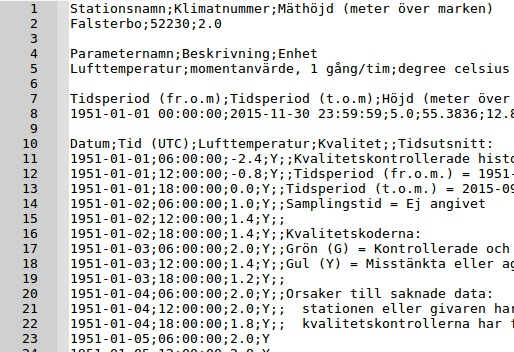
\includegraphics[width = \textwidth]{datastructure.jpg}
	  \caption{Data structure of the files used for analysis.}
	  \label{datastructure}
	 
	\end{figure}\noindent
	The first couple of lines consists of information which is irrelevant for reading in, which is why a for loop was used in order to skip the first lines until it reaches 
	the first data point, which can be identified by its ``year-month-day;hour:minute:second;temperature`` format.
	\\\\
	In order to obtain the information in each data point it was first split into three separate strings at each '';``. In the next step the ``year-month-day'' string was split 
	further at each ``-'' and stored into separate vectors. The same was done to the ``hour:minute:second'' string for each ``:'' and the hour was stored in a 
	vector (the data points contains no minutes or seconds and are thus not stored in vectors). Last step was to convert the temperature to a float and then store it in a vector. 
	\\\\
	The next step was to create a date vector which calculates the time in terms of year (in decimal) so that one can display all the data points in the same plot without having 
	for example data point ``1951-06-11 6:00:00`` and data point ``1951-06-11 12:00:00'' having the same x-value. The code itself converts hours, days and months into equivalent 
	amount of one year and adds it all together with the year and then stores the result in a vector. The code also checks if the current year is a leap year and then takes 
	into consideration the extra day when converting things to years.

\end{document}